%%%% Better Poster latex template example v1.0 (2019/04/04)
%%%% GNU General Public License v3.0
%%%% Rafael Bailo
%%%% https://github.com/rafaelbailo/betterposter-latex-template
%%%% 
%%%% Original design from Mike Morrison
%%%% https://twitter.com/mikemorrison

\documentclass[widescreen,fleqn]{betterposter}

%%%% Uncomment the following commands to customise the format

%% Setting the width of columns
% Left column
\setlength{\leftbarwidth}{0\paperwidth}
% Right column
\setlength{\rightbarwidth}{0.33\paperwidth}

%% Setting the column margins
% Horizontal margin
%\setlength{\columnmarginvertical}{0.05\paperheight}
% Vertical margin
%\setlength{\columnmarginhorizontal}{0.05\paperheight}
% Horizontal margin for the main column
\setlength{\maincolumnmarginvertical}{0.05\paperheight}
% Vertical margin for the main column
\setlength{\maincolumnmarginhorizontal}{0.05\paperheight}

%% Changing font sizes
% Text font
%\renewcommand{\fontsizestandard}{\fontsize{28}{35} \selectfont}
% Main column font
\renewcommand{\fontsizemain}{\fontsize{110}{130} \selectfont}
% Title font
\renewcommand{\fontsizetitle}{\fontsize{60}{35} \selectfont}
% Author font
\renewcommand{\fontsizeauthor}{\fontsize{40}{35} \selectfont}
% Section font
%\renewcommand{\fontsizesection}{\fontsize{28}{35} \selectfont}

%% Changing font sizes for a specific text segment
% Place the text inside brackets:
% {\fontsize{28}{35} \selectfont Your text goes here}

%% Changing colours
% Background of side columns
%\renewcommand{\columnbackgroundcolor}{black}
% Font of side columns
%\renewcommand{\columnfontcolor}{gray}
% Background of main column
%\renewcommand{\maincolumnbackgroundcolor}{empirical}
%\renewcommand{\maincolumnbackgroundcolor}{theory}
%\renewcommand{\maincolumnbackgroundcolor}{methods}
%\renewcommand{\maincolumnbackgroundcolor}{intervention}
% Font of main column
%\renewcommand{\maincolumnfontcolor}{gray}

\begin{document}	
\betterposter{
%%%%%%%% MAIN COLUMN

\maincolumn{
%%%% Main space
\begin{minipage}[t]{\textwidth}
    \begin{center}
        \textbf{Protein Tandem Repeats} (TRs) originate by duplication and are involved in "housekeeping" functions. \\
        \vspace{5mm}
        In viruses, TRs are found in proteins \textbf{essential for virulence}.
        \vspace{15mm}
        
        \begin{center}
            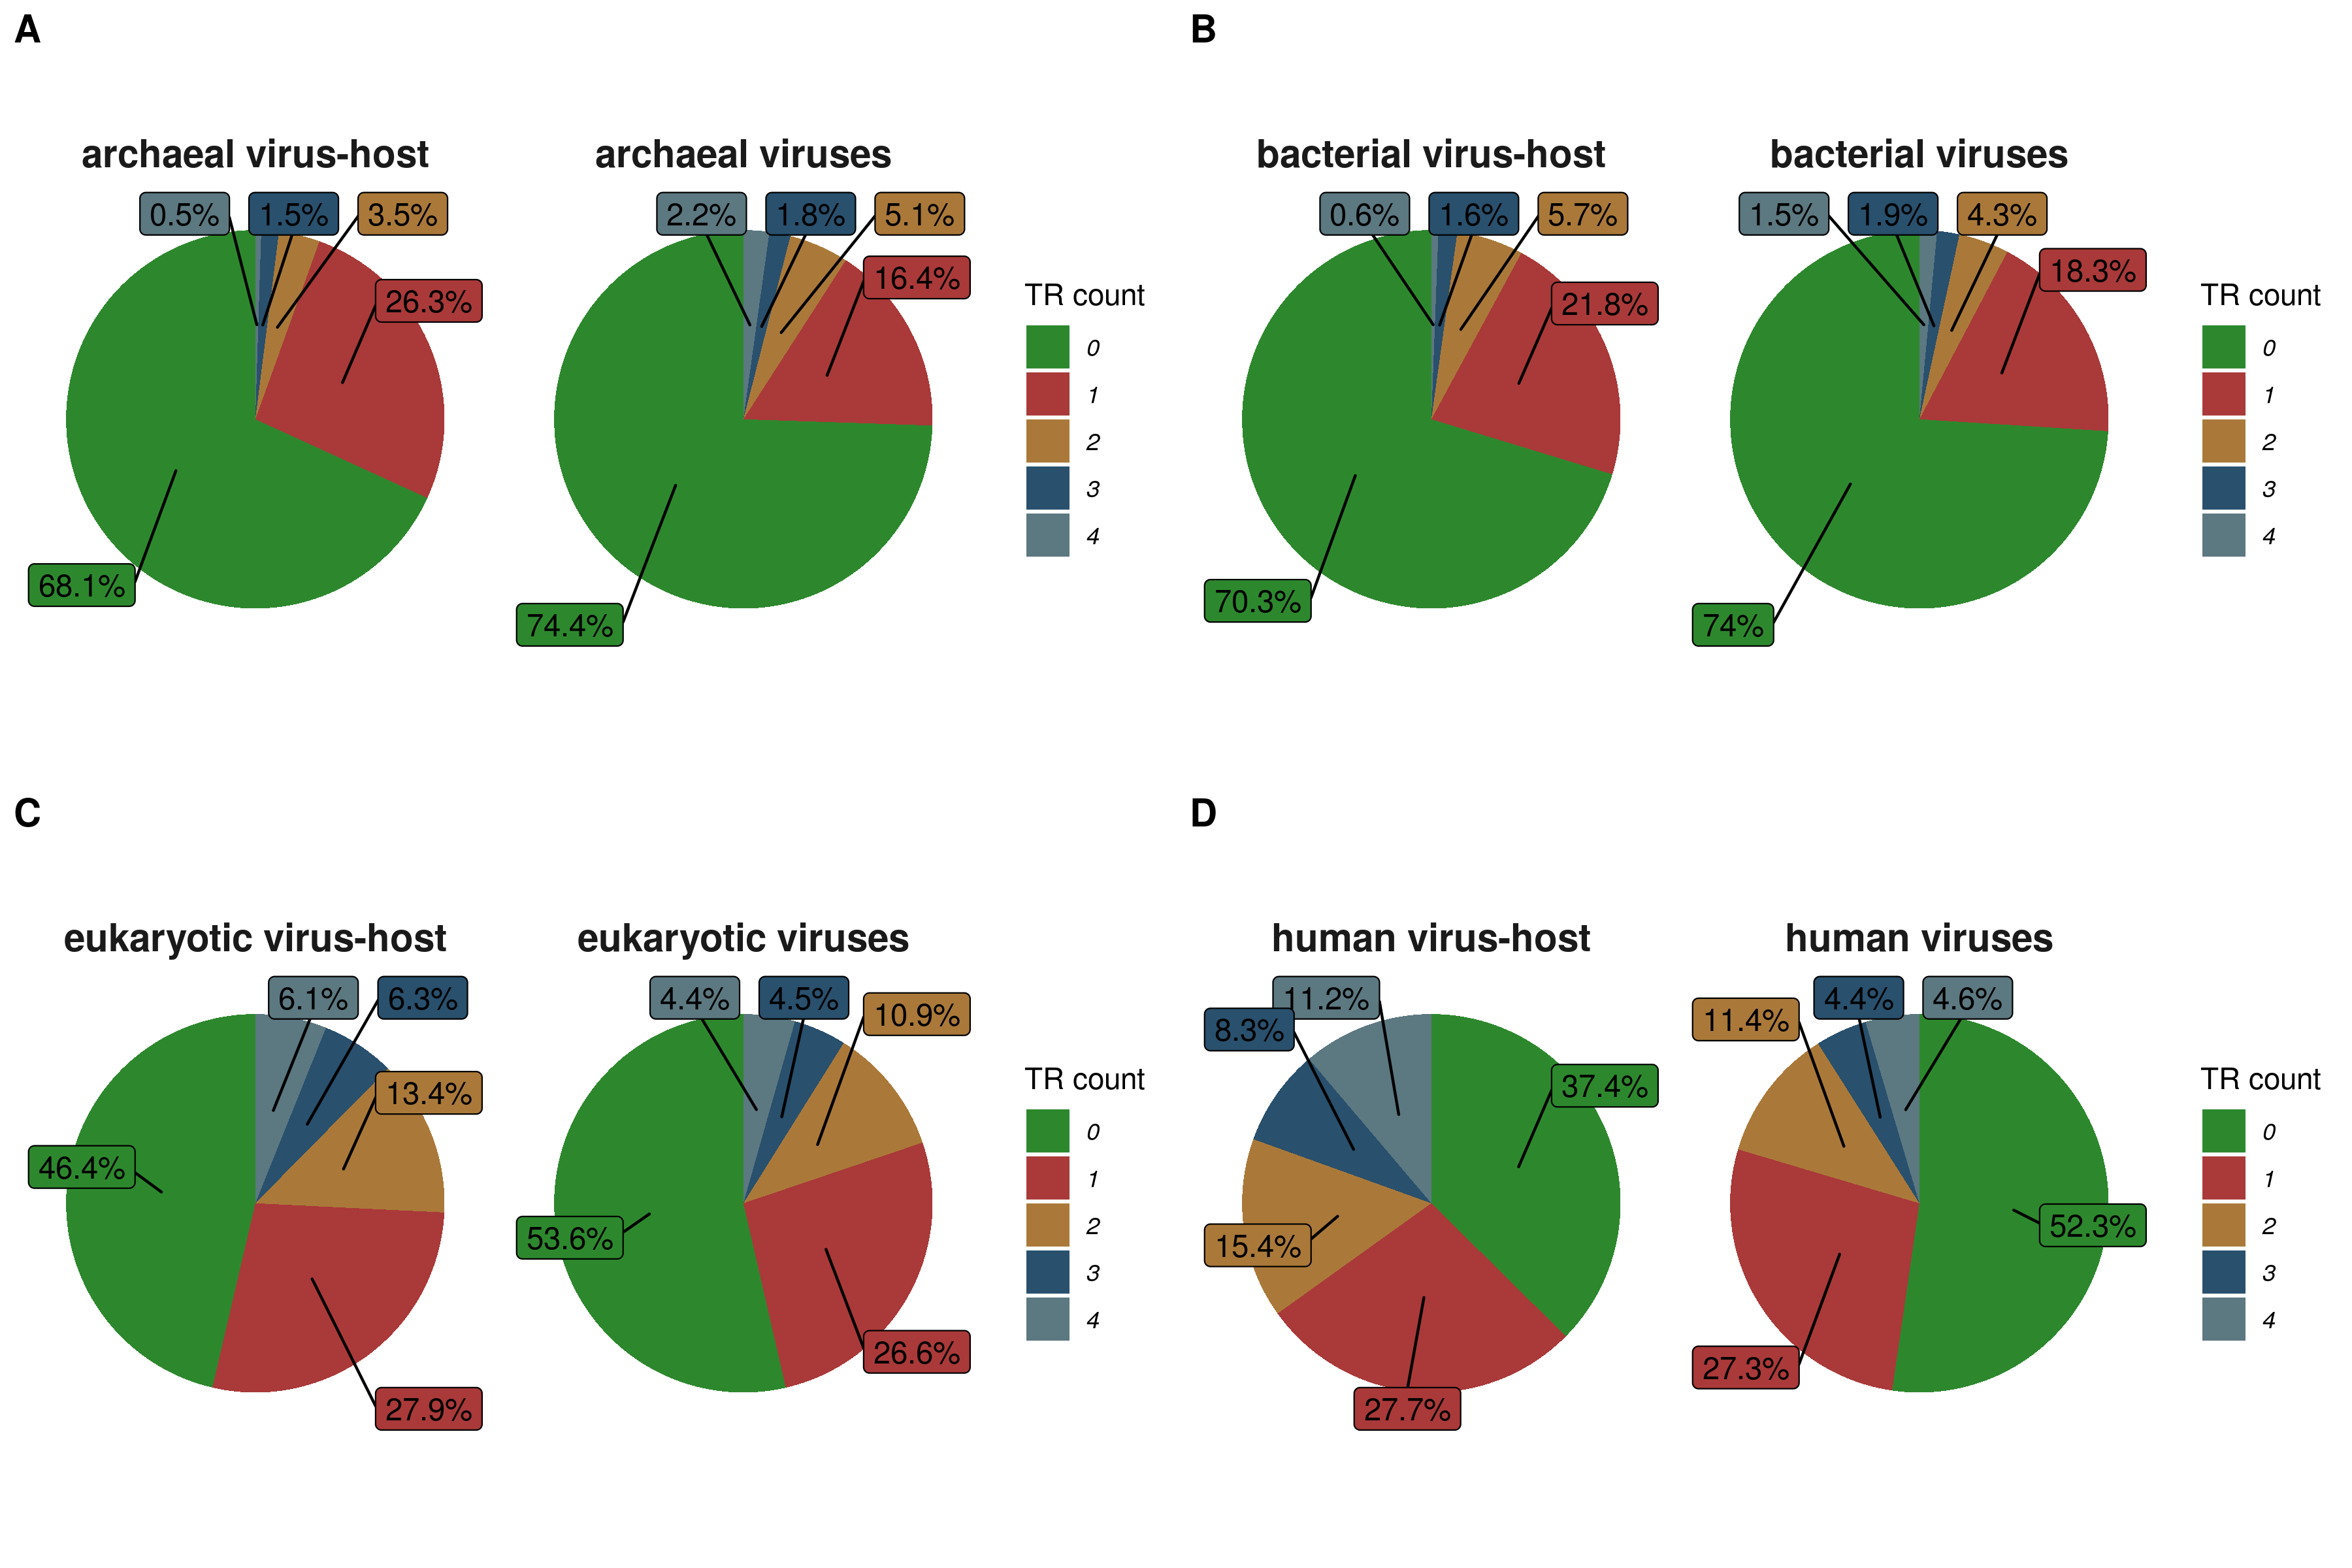
\includegraphics[width=0.6\textwidth]{figures/virus_virushost_cake_all.png}
        \end{center}        
    \end{center}
\end{minipage}

}{
%%%% Bottom space

%% Paper reference
\begin{minipage}[t]{\textwidth}
    \begin{center}
        {\fontsize{35}{35} \selectfont 
            Delucchi, M.; Schaper, E.; Sachenkova, O.; Elofsson, A.; Anisimova, M.
        }
        \\{\fontsize{45}{35} \selectfont 
            \textbf{A New Census of Protein Tandem Repeats and Their Relationship with Intrinsic Disorder.}
        }
        \\{\fontsize{35}{35} \selectfont 
            Genes 2020, 11, 407.
        }
    \end{center}
\end{minipage}

%% Institution logo and QR Code
\begin{minipage}[t]{\textwidth}
    \begin{center}
    \compactqrcode{img/qrcode}{}
    
\includegraphics[width=0.105\paperwidth]{img/zhaw_lsfm_ias_blau_en.jpg}
    
\includegraphics[width=0.05\paperwidth]{img/logo_SU.png}
    
\includegraphics[width=0.063\paperwidth]{img/logo_sib.png}    
    \end{center}
\end{minipage}

\begin{minipage}[t]{\textwidth}
    \begin{center}
        {\fontsize{35}{35} \selectfont 
            \href{mailto:matteo.delucchi@zhaw.ch}{matteo.delucchi@zhaw.ch}
        }
    \end{center}
\end{minipage}

}

}{
%%%%%%%% LEFT COLUMN
}{
%%%%%%%% RIGHT COLUMN

\begin{center}
    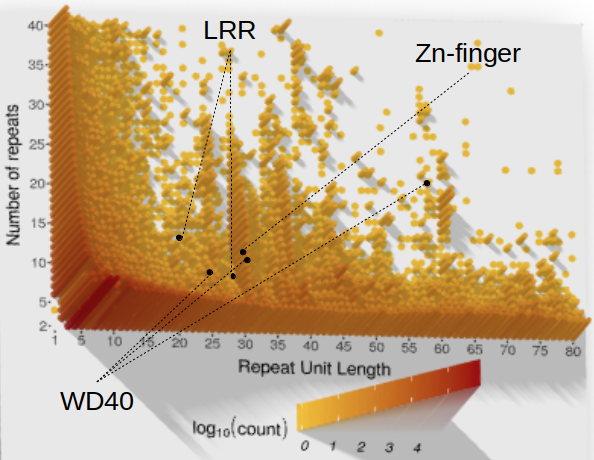
\includegraphics[width=0.35\textheight]{figures/fig1_3D_rotated.png}
\end{center}
Most of the known proteins contain TRs. A vast variation in TR lengths and unit copy numbers could be detected with a majority of proteins having >1 TR and a positive correlation between protein length and number of different TRs.
Viruses have fewer TRs compared to their host and complex organisms are enriched with TRs.

\begin{center}
    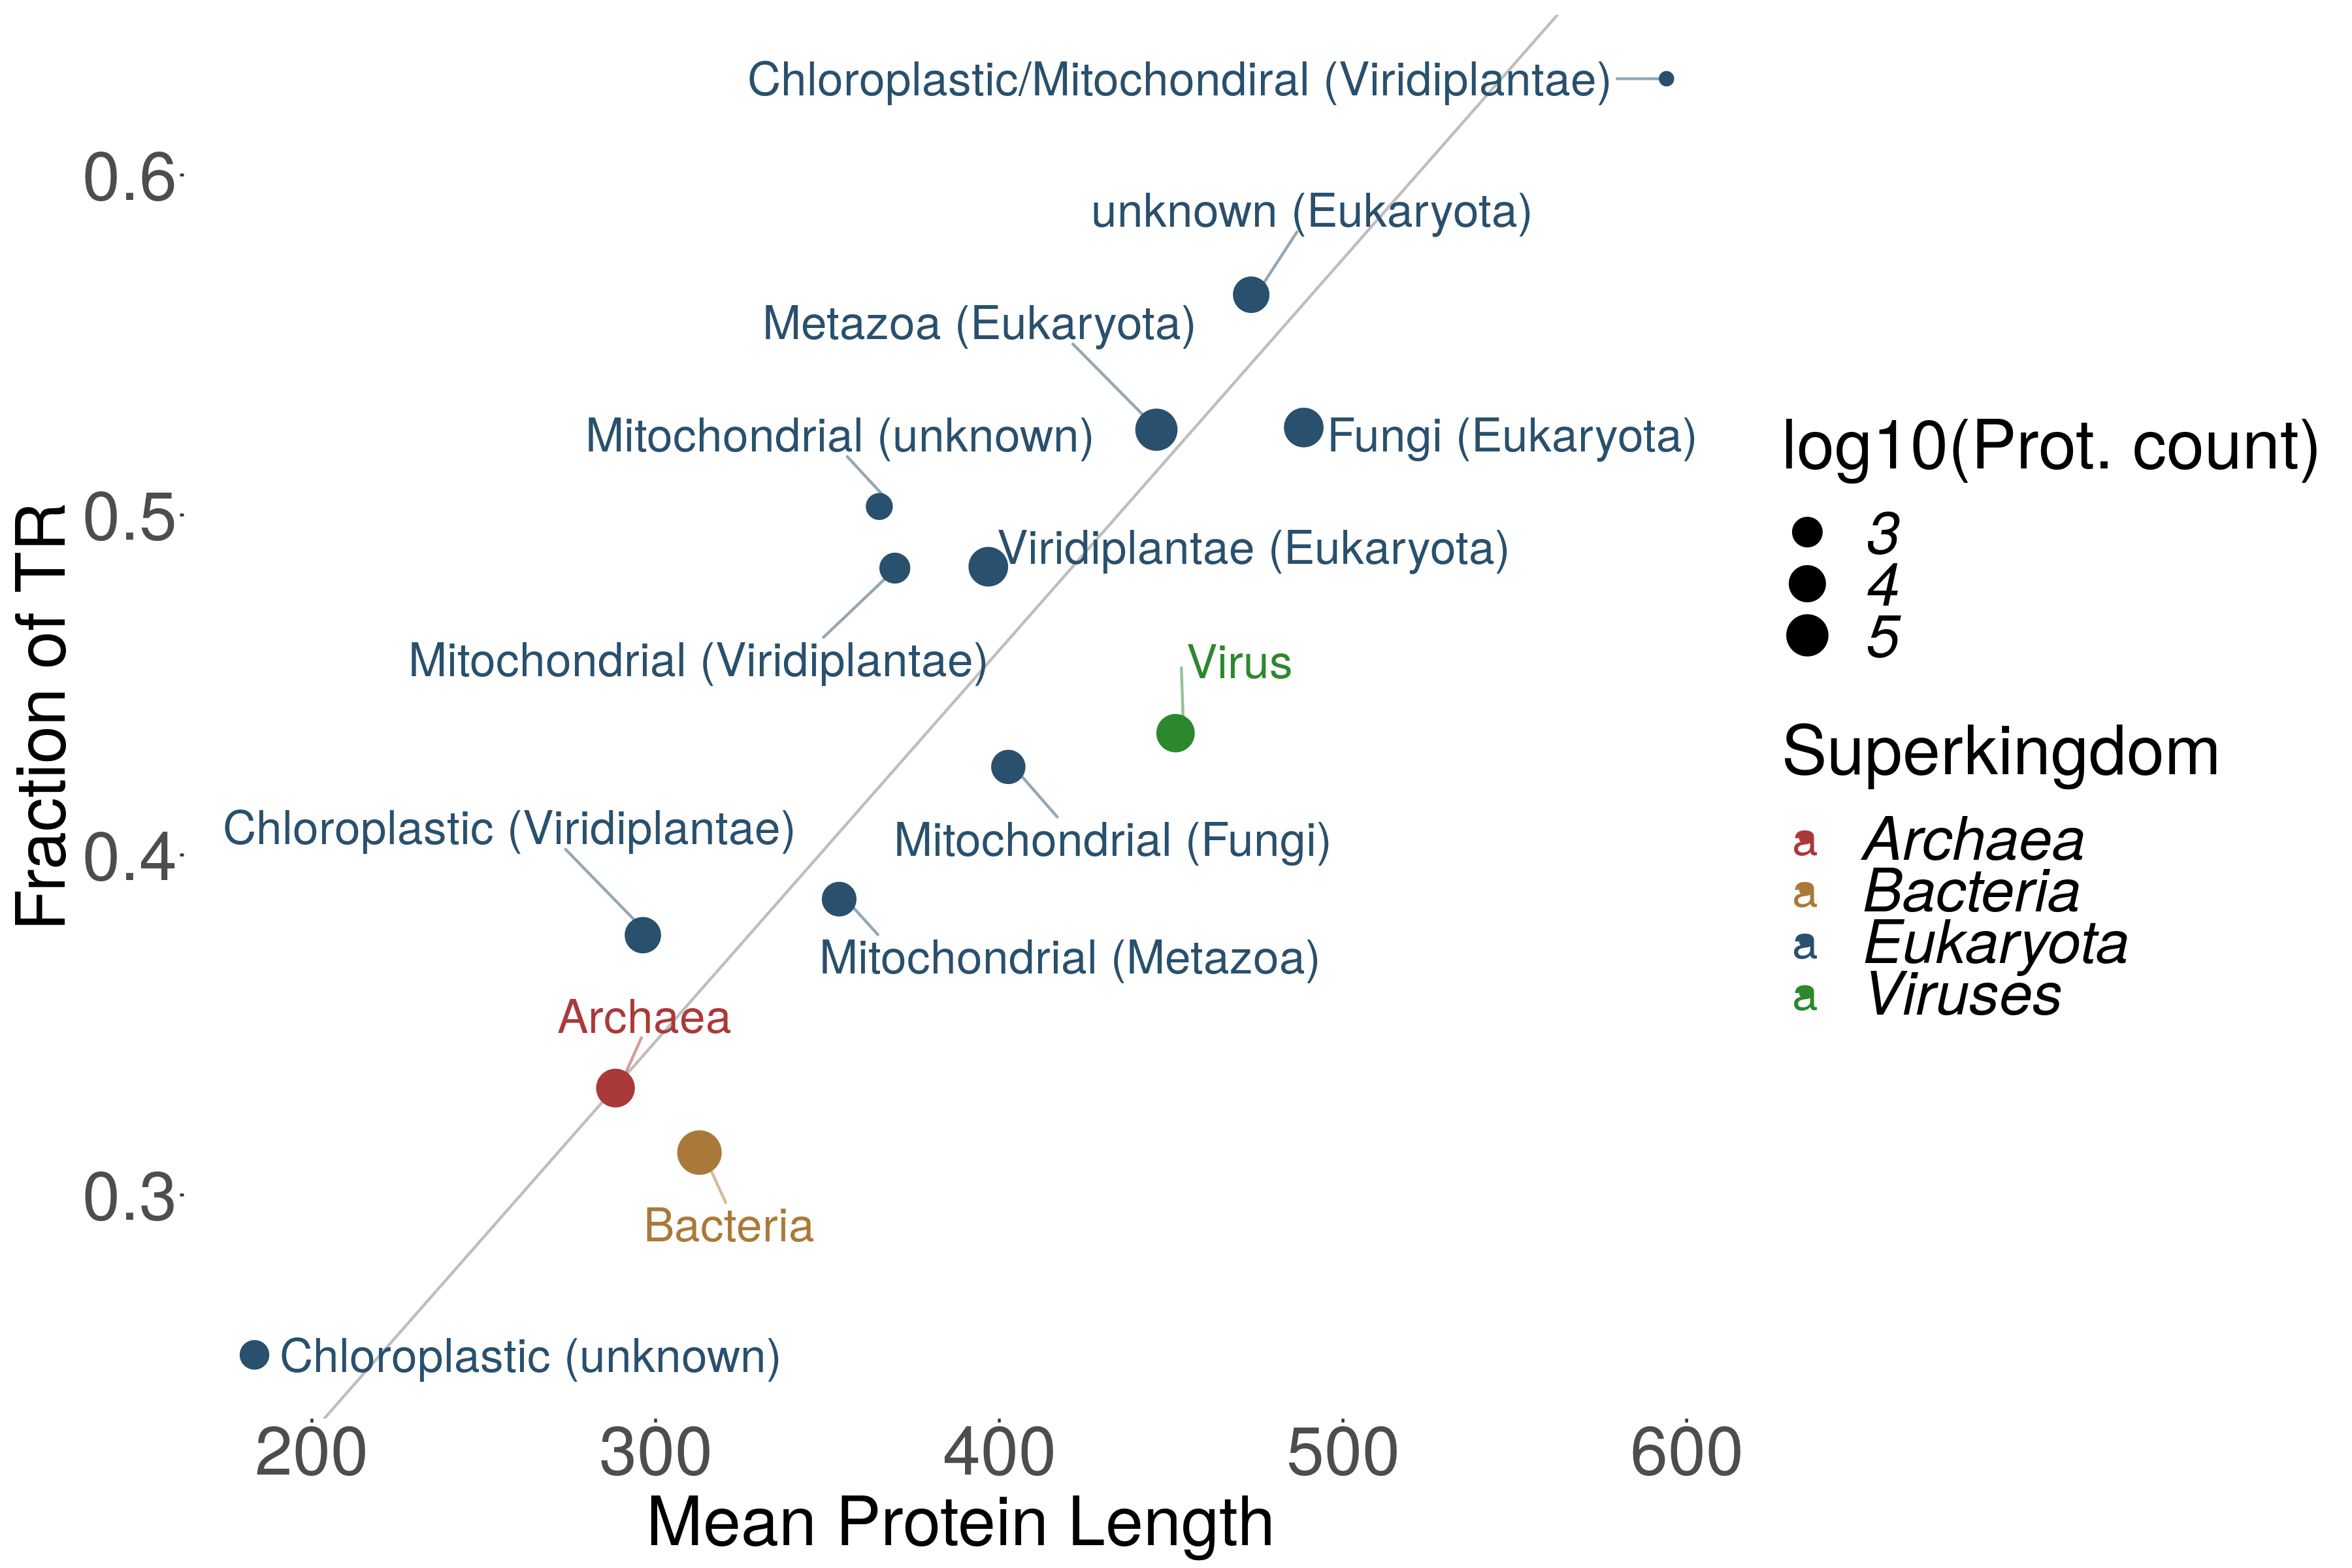
\includegraphics[width=0.4\textheight]{figures/Mean_Prot_length_vs_Frac_TR.png}
\end{center}
TR location is biased towards the sequence flanks for shorter TRs and they are enriched with disorder-promoting amino acids and are often found in proteins with intrinsic disorder regions.
TR containing proteins are involved in transcription processes, structural organization, electron transport
and ion-binding.

\begin{center}
    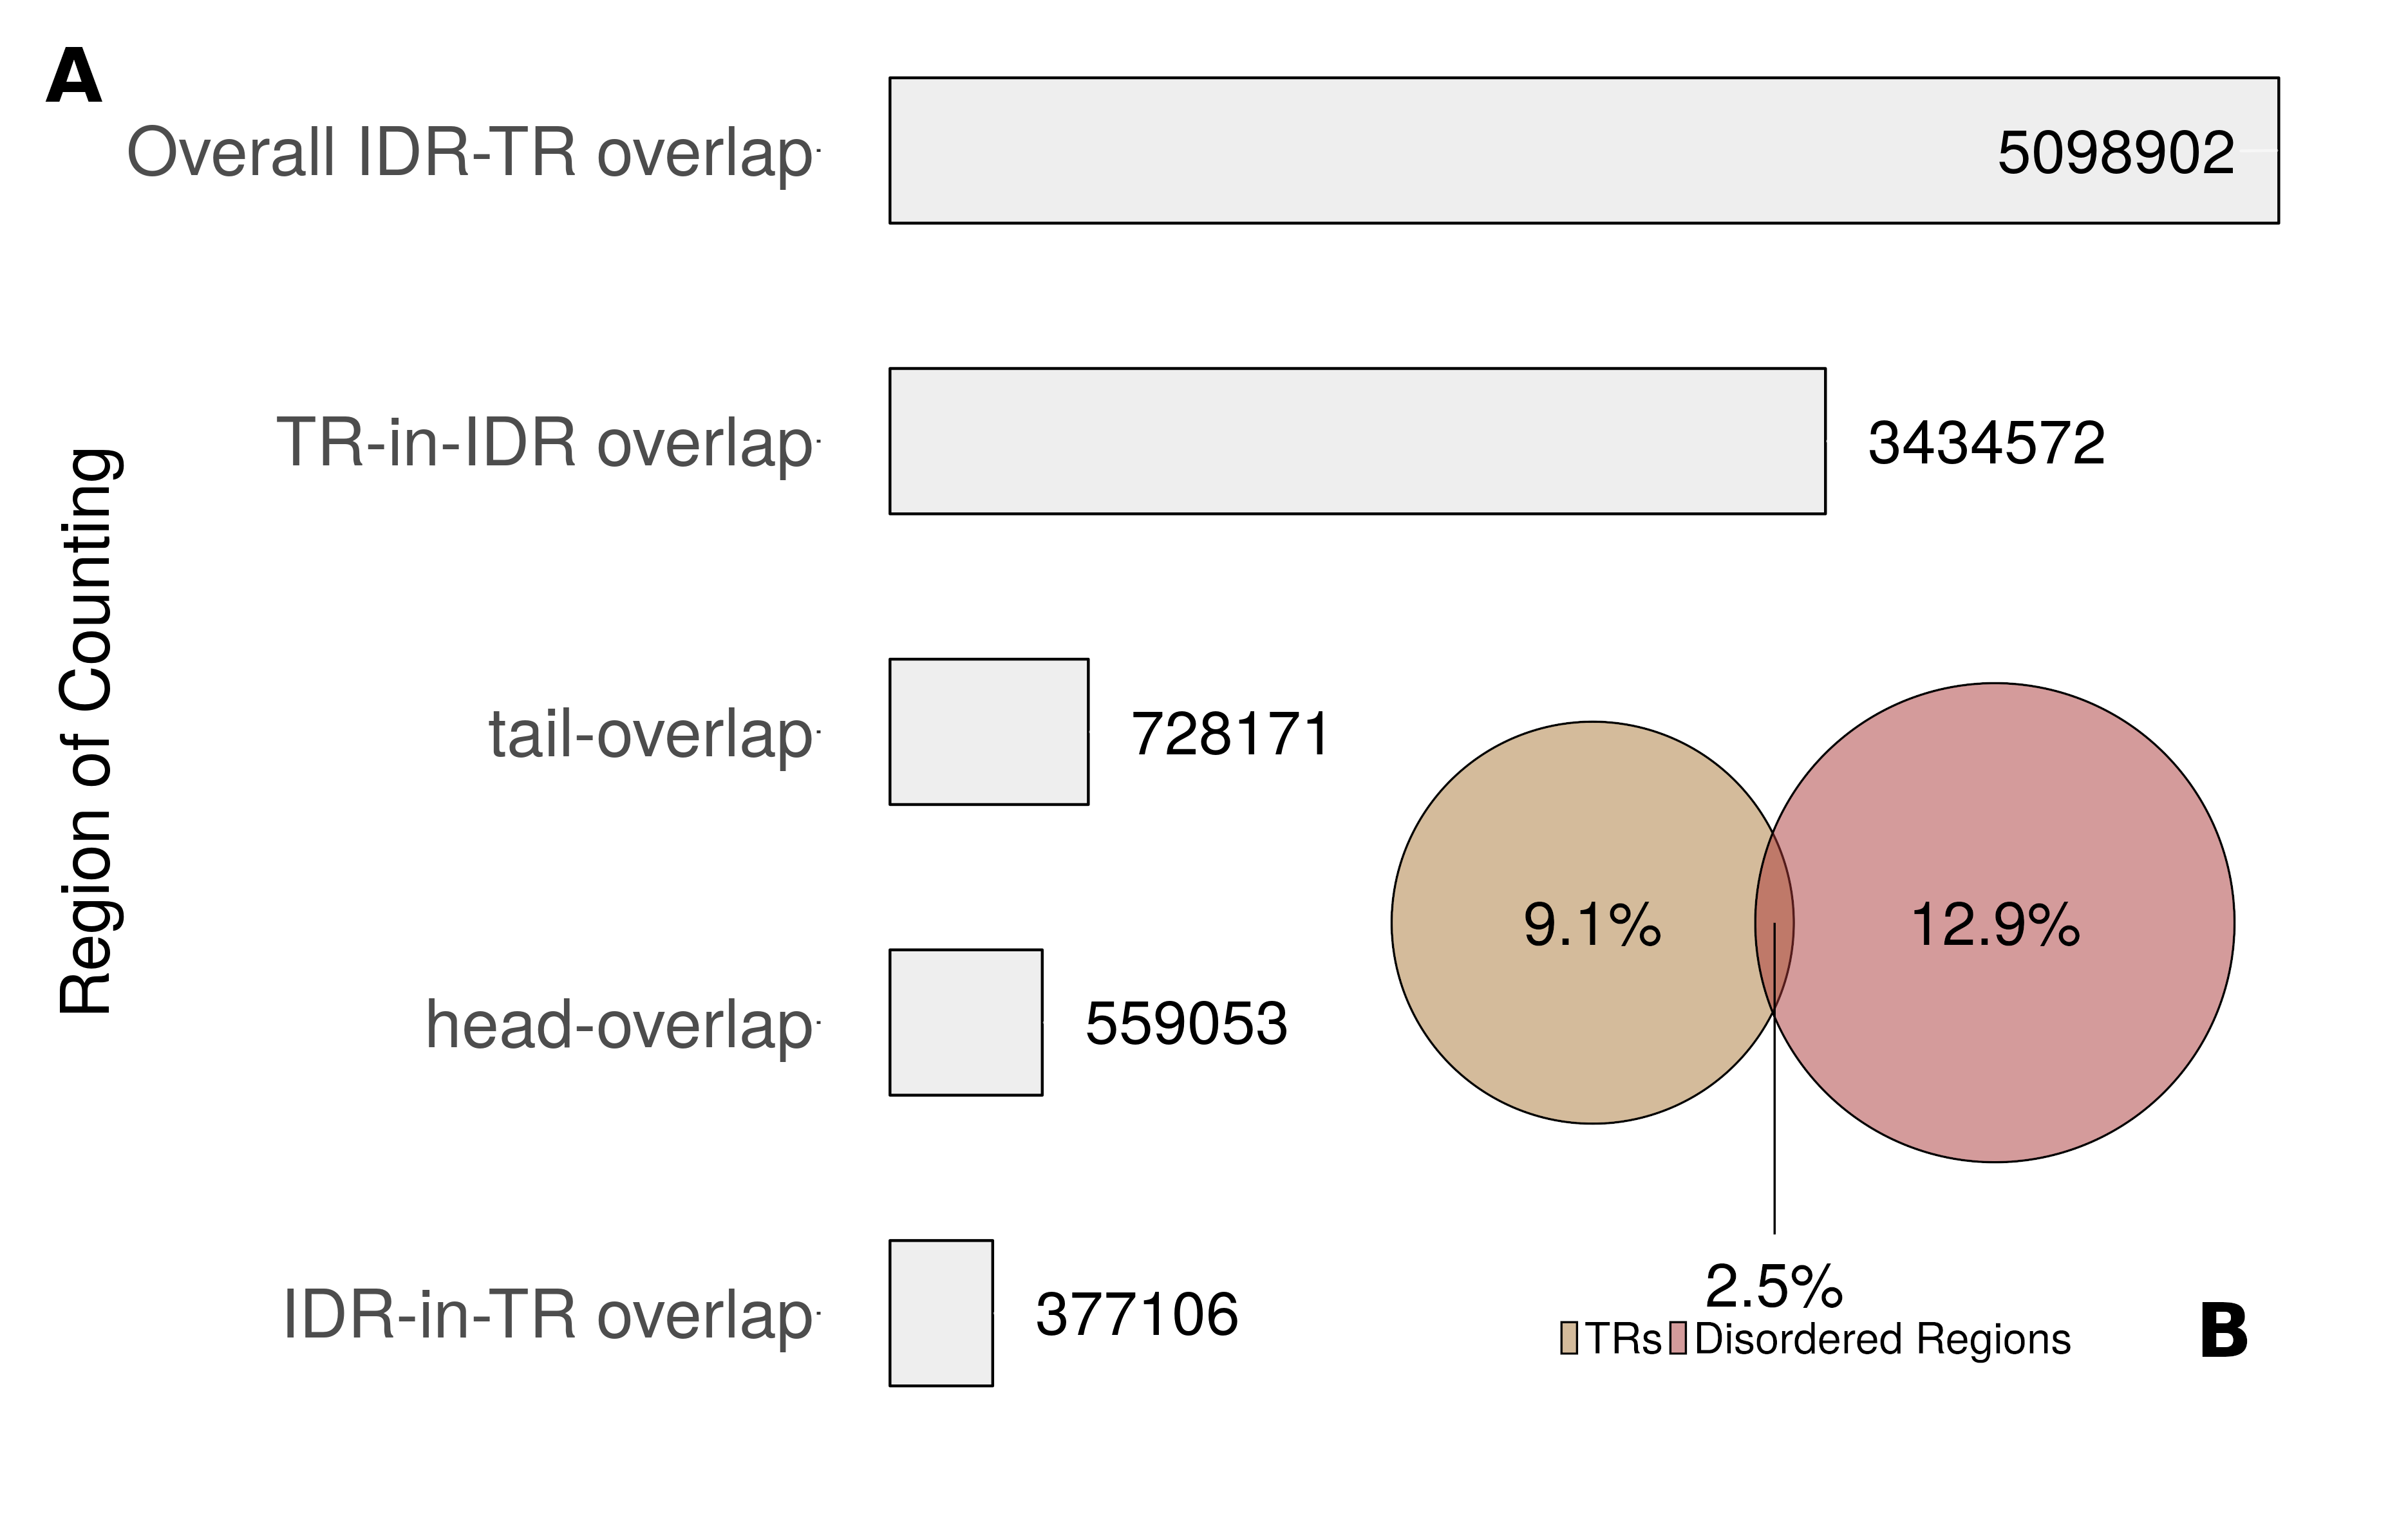
\includegraphics[width=0.4\textheight]{figures/TR_disorder_overlap_overall_detail_and_venn.png}
\end{center}

}
\end{document}